%!TEX root = ../../common/main.tex

\chapter{Conclusion and outlook}
\label{ch:conclusion}

After the first run of the \LHC and an efficient data taking period, the
foundation of the \SM remains solid. The discovery of the Higgs boson
\cite{Aad:2015zhl} endorses the theoretical framework and is a huge success for
the particle physics community. Still, the necessity of \BSM physics is not
deniable. Missing observations of \BSM effects like heavy super-symmetric
particles or a suitable dark matter candidate dash the hope of new findings at
the \si{TeV}-scale. \RunTwo of the \LHC will be crucial for the future of the
particle physics community and the design of next-generation experiments.

While direct searches for new heavy particles are constrained by the available
collision energies, indirect searches are sensitive to \BSM effects through
higher order contributions, even with collision energies far below the threshold
for direct production of heavy particles. The \LHCb experiment was therefore
designed to perform high precision tests of the \SM in decays of \B and \D
mesons and to identify possible deviations from the \SM. Especially the
measurement of \CP violation in the decay of \BdToJpsiKS acts as a poster child
with small theoretical uncertainties, easy to reconstruct final states, and high
event yields.

The measurement of the \CP parameters \SJpsiKS and \CJpsiKS presented in this
thesis is realised on a dataset corresponding to an integrated luminosity of
$\SI{3.0}{\per\femto\barn}$ recorded by the \LHCb experiment in
\acl{protonproton} collisions at centre-of-mass energies of $\num{7}$ and
$\SI{8}{\TeV}$. The sample contains $\num{41500}$ reconstructed $\BdToJpsiKS$
candidates with a flavour tagging decision assigned by the combination of the
\acl{OS} tagging algorithms or by the \acl{SSpi} tagging algorithm. Using an
\acl{uEML} fit, the \CP parameters \SJpsiKS and \CJpsiKS are measured to be
%
\begin{equation*}
  \begin{split}
    \SJpsiKS &= \phantom{-}\num{0.731} \pm \num{0.035} \statp \pm \num{0.020} \systp \eqcm\eqand \\
    \CJpsiKS &=           \num{-0.038} \pm \num{0.032} \statp \pm \num{0.005} \systp \eqcm
  \end{split}
\end{equation*}
%
with a statistical correlation coefficient of $\rho(\SJpsiKS,\CJpsiKS) =
\num{0.483}$. With the parameter \CJpsiKS fixed to zero, the measurement yields
%
\begin{equation*}
  \SJpsiKS = \sintwobeta = \num{0.746 +- 0.030}\statp \eqpd
\end{equation*}

The measurement improves the previous \LHCb result \cite{Aaij:1497268} by
including a larger dataset, additional trigger lines, an optimised candidate
selection and by incorporating the \SSpi tagger decisions. It is the most
precise measurement of \CP violation at a hadron collider and is in excellent
agreement with the current world average. 

Including this measurement, the updated world average on \sintwobeta
\cite{Amhis:2014hma} is
%
\begin{equation*}
  \sintwobeta = \num{0.691 +- 0.017} \eqcm
\end{equation*}
%
reducing the tension to the fit of all other \CKM matrix parameters slightly to
$\Delta\chisq = \num{1.66}$ \cite{Charles:2004jd}.
\Cref{fig:conclusion:ckm_fitter_15} shows the ${(\dquark,\bquark)}$ unitarity
triangle in the ${(\ovE{\rho},\ovE{\eta})}$-plane from a global fit
incorporating all measured \CKM parameters \cite{Charles:2004jd} except from the
one reported here that is additionally shown to allow for a better comparison.
%
\begin{figure}[ht]
\centering
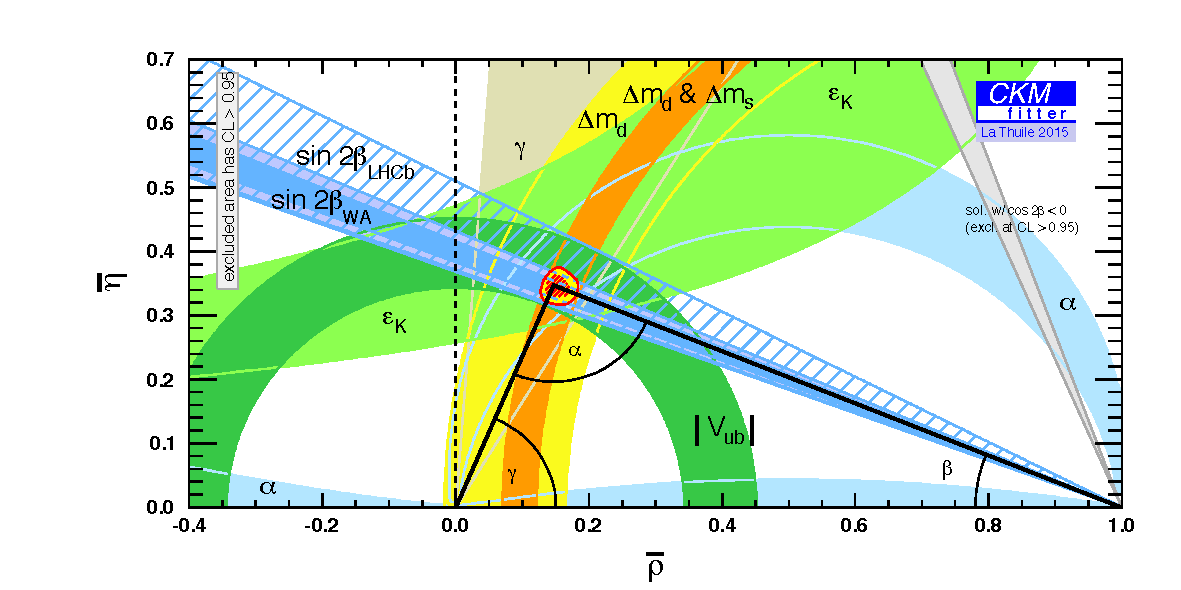
\includegraphics[width=1\textwidth]{private/content/conclusions/figs/ckmfitter_summer15.pdf}
\caption{Constraints on the ${(\dquark,\bquark)}$ unitarity triangle in the
${(\ovE{\rho},\ovE{\eta})}$-plane from a global fit incorporating all measured
\CKM parameters except the results presented in this thesis, which is shown
separately as a comparison in light blue. Regions outside the coloured areas
have $1-p > \SI{95.45}{\percent}$. The red hashed region of the global
combination corresponds to $\SI{68}{\percent}$ \acp{CL}. \cite{Charles:2004jd}}
\label{fig:conclusion:ckm_fitter_15}
\end{figure}

During \RunTwo of the \LHC, starting this year at a centre-of-mass energy of
$\SI{13}{\TeV}$, \LHCb is expected to collect a large dataset corresponding to
an integrated luminosity of around $\SI{5}{\per\femtobarn}$ until the next long
shut-down scheduled in 2018. With an estimated sensitivity on \SJpsiKS of
$\num{0.018}$ \cite{Moedden:2015}, this additional data will allow the \LHCb
collaboration to perform the world's best single measurement of \sintwobeta. As
this sensitivity falls below the current systematic uncertainty, an emphasis has
to be laid on a better understanding of the background tagging asymmetry and to
reduce the uncertainties on the flavour tagging calibration parameters. With
more data being available, a reassessment of the magnitude of the background
tagging asymmetry is possible, leading either to a model to describe the effect
inside the likelihood fit or a confirmation that no background asymmetry is
present in data. The uncertainties on the flavour tagging parameters will shrink
with more data available in the calibration and cross-check channels, as well as
a better understanding of the flavour tagging algorithms and new developments in
the calibration procedure. Furthermore, the systematic uncertainty due to
neglecting the decay width difference \DGd will become closer to the statistical
uncertainty in \RunTwo, such that the handling of \DGd has to be revisited
\cite{Moedden:2015}.

To further improve the sensitivity on the measurement of \sintwobeta, additional
decay modes will be explored. Based on the \RunOne dataset, the decay of the \Bd
into the $\Jpsi (\to\elel) \KS$ final state is expected to contribute with a
sensitivity of $\num{0.1}$ \cite{bdtojpsieeks:ramon}. Beyond that, higher
charmonium resonances as in $\BdToPsiTwoSKS$ will add sensitivity to the
combined result. Preparatory studies have shown an expected sensitivity on
\sintwobeta of $\num{0.09}$ in the combination of the $\psitwos\to\Jpsi\pi\pi$
and the $\psitwos\to\mumu$ final states for \RunOne \cite{Mueller:2014}.

The biggest \LHCb competitor will be the \BelleTwo experiment. The collaboration
plans to start data taking in 2018 with an expected instantaneous luminosity
$\num{50}$ times larger than its precursor \Belle. With an assumption of
$\num{100}$ days of efficient data taking per year, an integrated luminosity of
$\SI{8}{\per\attobarn}$ will be recorded per year. If these expectations hold
true, \BelleTwo will be able to reduce the total uncertainty on \sintwobeta to
$\num{0.010}$ on a short time scale with the uncertainty mainly being dominated
by irreducible systematic uncertainties \cite{Aushev:2010bq}.

During the second long shut down of the \LHC in 2018 the \LHCb detector will be
upgraded to cope with a higher instantaneous luminosity of $L =
\SI{2e33}{\lumi}$ and an enhanced $\bquark\bquarkbar$-pair production rate of
$\num{e6}$ per second \cite{Bediaga:1443882}. The upgrade involves a new hybrid
pixel sensor \VELO \cite{TDRVELO}, new tracking stations based on silicon
micro-strip and scintillating fibre technology \cite{TDRTracking}, enhancements
of the \RICH systems, the calorimeters and the muon system \cite{TDRPID}, and a
new software trigger concept capable to read out the full detector at the
nominal bunch crossing frequency of $\SI{40}{\mega\hertz}$ \cite{TDRTrigger}.
These actions will result in an large dataset corresponding to an expected
integrated luminosity of $\SI{50}{\per\fb}$ with the upgraded detector. Assuming
unchanged data taking efficiencies and similar performance of the trigger,
stripping, and flavour tagging, \ToyMC studies estimate a sensitivity on
\sintwobeta of around $\num{0.007}$ \cite{Moedden:2015} in the decay
\BdToJpsiKS.
